% !TeX program = lualatex
% !TeX encoding = utf8
% !TeX spellcheck = uk_UA
% !BIB program = bibler

\documentclass[]{beamer}
\usetheme{Electromagnetism}



\usepackage{Electromagnetism}
\hypersetup{
  colorlinks=true,
  linkcolor=cyan,  % Цвет для внутренних ссылок
  urlcolor=red,    % Цвет для URL
  citecolor=blue   % Цвет для библиографических ссылок
}




%============================================================================
\title[Лекції електрики та магнетизму]{\huge\bfseries Діелектрики \\ в електричному полі}
\subtitle{Лекції з електрики та магнетизму}
\author{Пономаренко С. М.}
\date{}
%============================================================================
\graphicspath{{pictures/}}
\begin{document}


\begin{frame}[plain]
	\maketitle
	%	\tikz[remember picture,overlay] \node[opacity=0.7,inner sep=0pt,
	%		anchor=north west] at (current page.north
	%	west){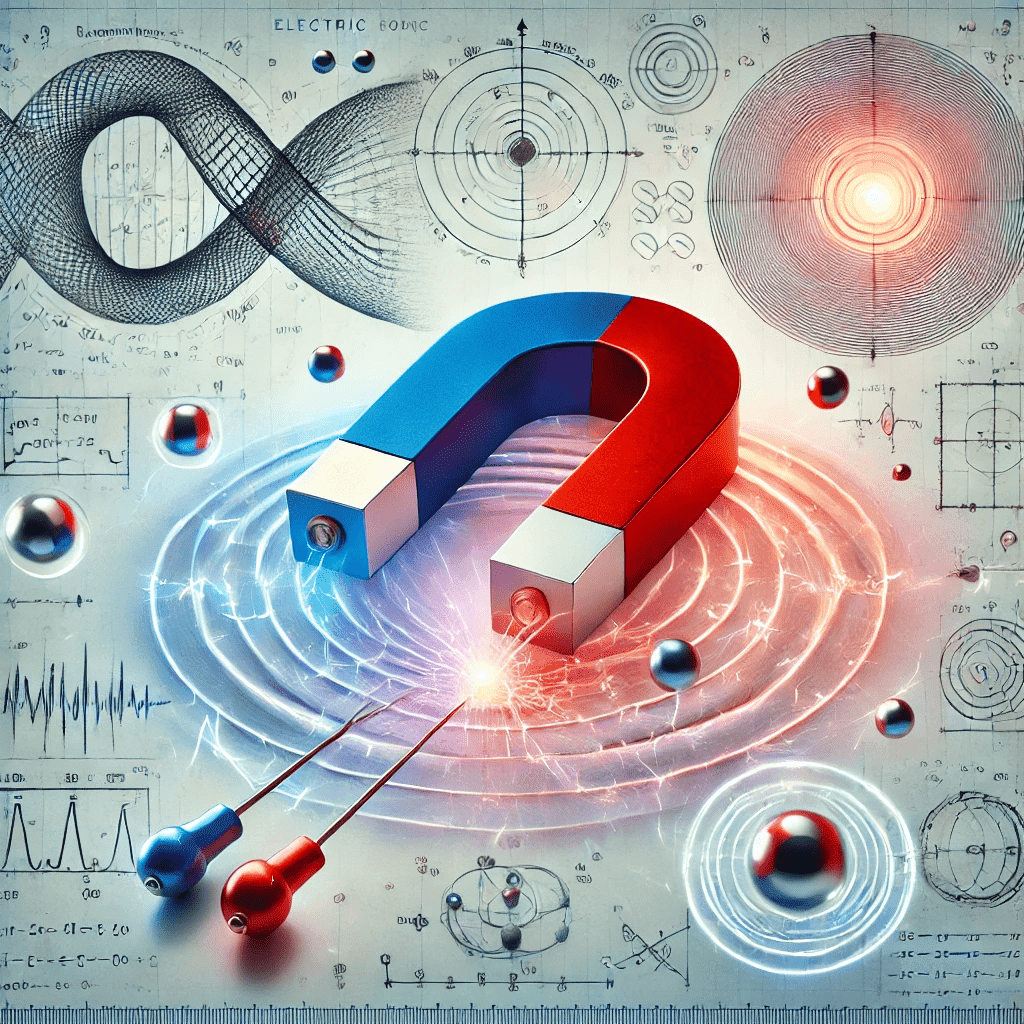
\includegraphics[width=2cm]{EMInteractions}};
\end{frame}

% ============================== Слайд ## ===================================
\begin{frame}{Зміст лекції}{}
	\tableofcontents
\end{frame}
% ===========================================================================

%% --------------------------------------------------------
\section{Основні поняття}
%% --------------------------------------------------------



% ============================== Слайд ## ===================================
\begin{frame}{Основні поняття}{}\small

	\begin{block}{}\justifying
		\alert{Вільні заряди} --- це заряди, які можуть переміщатися на великі відстані в речовині
		(набагато більші за міжатомні відстані). У діелектриках вільних зарядів, як правило, мало.

		\smallskip

		\alert{Зв'язані (поляризаційні) заряди} --- це заряди, які під дією зовнішніх полів або сил мало
		зміщуються відносно свого положення рівноваги і повертаються назад, у положення рівноваги, після
		зняття
		зовнішнього впливу.

		\smallskip

		\alert{Діелектриками} називають речовини, в структурі яких є зв'язані заряди, вільних зарядів дуже
		мало, або зовсім нема.

	\end{block}

	\begin{block}{}\justifying\scriptsize
		\alert{Мікрополе} $\Efield_\text{micro}$ --- це результат додавання полів багатьох
		зарядів. Це поле
		швидко змінюється від точки до точки і в часі.

		\smallskip

		\alert{Середнє поле} $\left\langle \Efield\right\rangle$  --- це результат усереднення
		мікрополя по
		фізично нескінченно малому об'єму $\Delta V$. Це поле змінюється істотно повільніше, ніж
		мікрополе:
		\begin{equation*}
			\left\langle \Efield\right\rangle = \frac1{\Delta V} \iiint\limits_{\Delta V}
			\Efield_\text{micro} dV.
		\end{equation*}
	\end{block}
\end{frame}
% ===========================================================================

%% --------------------------------------------------------
\section{Структура діелектриків}
%% --------------------------------------------------------


% ============================== Слайд ## ===================================
\begin{frame}{Дипольні моменти деяких полярних молекул}

	\begin{block}{}\justifying\small
		Дипольний момент виникає внаслідок різної електронегативності атомів, що складають
		молекулу, та
		розташуванню їх в просторі.
	\end{block}
	\begin{block}{}\justifying\scriptsize
		Дебай (позначається як \textit{Д} або \textit{D}) --- позасистемна одиниця вимірювання
		електричного дипольного моменту молекул. Одиниця виміру названа на честь фізика П. Дебая.
		\begin{equation*}
			1\ \text{Дебай} = 10^{-18}\ \text{Фр}\cdot\text{см}.
		\end{equation*}
		Більшість полярних молекул має дипольний момент порядку $1$ Д. Одиниця застосовується у
		фізичній хімії, атомній і молекулярній фізиці.
	\end{block}

	\begin{overprint}\centering\small
		\onslide<1>
		\begin{columns}
	\begin{column}{0.5\linewidth}\centering
		\begin{tikzpicture}[>=latex]
			\node[circle, draw=blue, ball color=blue!50, inner sep=0.28cm, text=blue] (O) at
			(0,0)
			{\tikz\draw[blue, thick] (0,0) -- ++(0.4, 0);};
			\node[below=15pt] at (O) {\ce{O^{2-}}};
			\node[circle, draw=red, ball color=red!50, inner sep=0.16cm, text=blue] (H1) at
			({90+105/2}:1)
			{$+$};
			\node[left=15pt] at (H1) {\ce{H^{+1}}};
			\node[circle, draw=red, ball color=red!50, inner sep=0.16cm, text=blue] (H2) at
			({90-105/2}:1)
			{$+$};
			\node[right=15pt] at (H2) {\ce{H^{+1}}};
			\draw[dashed, gray] (0, 0) -- ({90+105/2}:2);
			\draw[dashed, gray] (0, 0) -- ({90-105/2}:2);

			\draw[<->] (0, 0) ++({90-105/2}:1.8) arc({90-105/2}:{90+105/2}:1.8) node[pos=0.5,
					fill=white,
					font=\scriptsize]
				{$105^\circ$};

			\draw[->, red, ultra thick] (0,0) -- ++(0, 1.5) node[right] {$\vect{p}$};
		\end{tikzpicture}
        \begin{block}{}\footnotesize\centering
            Дипольний момент молекули \ce{H2O} $p = 1.84$ D
        \end{block}
	\end{column}
	\begin{column}{0.5\linewidth}\centering
    \begin{tikzpicture}[>=latex]
            \node[circle, draw=blue, ball color=blue!50, inner sep=0.28cm, text=blue] (N) at
			(0,0) {\tikz\draw[blue, thick] (0,0) -- ++(0.4, 0);};
        \node[above=15pt] at (N) {\ce{O}};
        \node[circle, draw=red, ball color=red!50, inner sep=0.16cm, text=blue] (H1) at
   				(225:1.2) {$+$};
        \node[circle, draw=red, ball color=red!50, inner sep=0.16cm, text=blue] (H2) at
			(280:1.8) {$+$};
        \node[circle, draw=red, ball color=red!50, inner sep=0.16cm, text=blue] (H3) at
   				(-45:1.2) {$+$};
        \draw[thick] (O) -- (H1) (O) -- (H2) (O) -- (H3);
        \draw[dashed] (H1) -- (H2) -- (H3) -- (H1);
       	\draw[->, red, ultra thick] (0,0) -- ++(0, -1.2) node[left] {$\vect{p}$};
    \end{tikzpicture}
        \begin{block}{}\footnotesize\centering
            Дипольний момент молекули \ce{NH3} $p = 1.46$ D
        \end{block}
	\end{column}
\end{columns}
		\onslide<2>
		\begin{tblr}{
			colspec={X[c, m]X[c,m]},
			row{1} = {c, m, fg=white, bg=cyan},
			hlines,
			vlines
			}
			Молекула                   & Дипольний момент (Дебай) \\
			Вода (\ce{H2O})            & 1.84                     \\
			Аміак (\ce{NH3})           & 1.46                     \\
			Вуглекислий газ (\ce{CO2}) & 0.00                     \\
			Хлороводень (\ce{HCl})     & 1.08                     \\
			Метанол (\ce{CH3OH})       & 1.70                     \\
		\end{tblr}
	\end{overprint}
\end{frame}
% ===========================================================================



% ============================== Слайд ## ===================================
\begin{frame}{Виникнення дипольного моменту неполярних молекул}
	\begin{block}{}\justifying\small
		\alert{Неполярні молекули} --- це молекули, в яких електричні заряди розподілені
		рівномірно, і
		відсутній постійний дипольний момент. У таких молекулах атоми зазвичай мають однакову або
		близьку електронегативність, тому електрони діляться рівномірно між атомами.
	\end{block}

	\begin{columns}
		\begin{column}{0.5\linewidth}\centering
			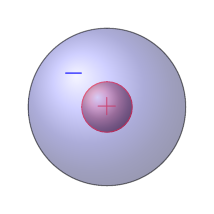
\begin{tikzpicture}
				\node[circle, draw=red, ball color=red!50, inner sep=0.1cm, text=red] (O) at (0,0)
				{$+$};
				\draw[ball color=blue!50, opacity=0.5] (O) circle (1);
				\node[text=blue] at (135:0.6) {$-$};
			\end{tikzpicture}
			\begin{block}{}\centering\scriptsize
				Дипольний момент без зовнішнього поля $p = 0$.
			\end{block}
		\end{column}
		\begin{column}{0.5\linewidth}
			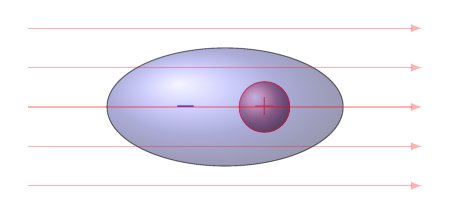
\begin{tikzpicture}[>=latex]
				\node[circle, draw=red, ball color=red!50, inner sep=0.1cm, text=red] (O) at (0,0)
				{$+$};
				\draw[ball color=blue!50, opacity=0.5] ([xshift=-0.5cm]O) ellipse (1.5 and 0.75);
				\node[text=blue] at (180:1) {$-$};

				\foreach \y in {-1,-0.5,...,1}
					{
						\draw[->, red, opacity=0.3] (-3, \y) -- ++(5, 0);
					}
			\end{tikzpicture}
			\begin{block}{}\centering\scriptsize
				Дипольний момент виник під дією зовнішнього поля $p \neq 0$.
			\end{block}
		\end{column}
	\end{columns}
	\begin{block}{} \justifying\small
		Прикладом неполярних молекул є кисень (\ce{O2}), азот (\ce{N2}), метан (\ce{CH4}) атоми
		інертних газів.
	\end{block}
\end{frame}
% ===========================================================================



% ============================== Слайд ## ===================================
\begin{frame}{Поляризація діелектриків}{}\small%
	\framesubtitle<1,2>{Полярні діелектрики}%
	\framesubtitle<3,4>{Неполярні діелектрики}%
	\framesubtitle<5,6>{Вектор поляризації}%
	\vspace*{-2em}
	\begin{overprint}
		\onslide<1-6>
		\begin{block}{}\justifying\small
			\alert{Поляризація} --- це просторовий \alert{перерозподіл зв'язаних зарядів}, що
			призводить до виникнення об'ємного дипольного моменту середовища. Поляризація може виникати
			як під дією електричних полів, так і під впливом інших зовнішніх чинників.
		\end{block}
	\end{overprint}
	\begin{overprint}
		\onslide<1,2>
		\begin{block}{}
			\alert{Полярні діелектрики} --- складаються з полярних молекул, що мають дипольний
			момент.
		\end{block}
		\onslide<3,4>
		\begin{block}{}
			\alert{Неполярні діелектрики} --- складаються з неполярних молекул, у яких центри
			позитивного і негативного зарядів збігаються.
		\end{block}
		\onslide<5>
		\begin{block}{}
			%            В обох випадках, на поверхні виділеного паралелепіпеда з'являються надлишкові
			%            (некомпенсовані) зв'язані заряди.
			%
			%            \smallskip
			\alert{Вектор поляризації (поляризованість)} --- це дипольний момент одиниці об'єму
			речовини (густина
			дипольного моменту):
			$
				\vect{P} = \dfrac1V \sum \vect{p}_i
			$
		\end{block}
		\onslide<6>
		\begin{block}{}
			В діелектрику сумарне поле, яке є суперпозицією зовнішнього поля $\Efield_\text{ex}$ і поля
			$\Efield'$ зв'язаних зарядів $\Efield = \Efield_\text{ex} + \Efield'$, ослаблюється.
		\end{block}
	\end{overprint}
	\begin{center}
		\begin{tikzpicture}[>=latex]
			\pgfmathsetseed{1}
			\tikzset{
				water/.pic={
						\begin{scope}[opacity=0.4]
							\node[circle, ball color=blue, inner sep=0, minimum size=0.3cm] (O) at
							(0,0) {};
							\node[circle, ball color=red, inner sep=0, minimum size=0.2cm] (H1) at
							(-50:0.2) {};
							\node[circle, ball color=red, inner sep=0, minimum size=0.2cm] (H2) at
							(50:0.2) {};
						\end{scope}
						\draw[-latex, brown, line width=1pt] (O) -- ++(0.5, 0);
					},
				unperturbed/.pic={
						\begin{scope}[opacity=0.4]
							\node[circle, ball color=blue, inner sep=0, minimum size=0.5cm] (O) at
							(0,0) {};
							\node[circle, ball color=red, inner sep=0, minimum size=0.2cm] (H1) at
							(0,0) {};
						\end{scope}
					},
				perturbed/.pic={
						\begin{scope}[opacity=0.4]
							\node[ellipse, ball color=blue, inner sep=0, minimum width=0.6cm,
								minimum
								height=0.4cm] (O) at
							(-0.1,0) {};
							\node[circle, ball color=red, inner sep=0, minimum size=0.2cm] (H1) at
							(+0.02,0) {};
						\end{scope}
						\draw[-latex, brown, line width=1pt] (-0.2,0) -- ++(0.5, 0);
					},
			};
			\uncover<1>{
				\foreach \x in {0,...,10}
					{
						\foreach \y in {0,...,3}{
								\pic[rotate={random(0,360)}] at ({0.75*\x}, {0.75*\y}) {water};
							}
					}
			}
			\uncover<2>{
				\foreach \y in {0,...,4} {
						\draw[->, red, thick] (-0.5,{0.75*\y-0.325}) -- ++(8.75,0);
					}
				\foreach \x in {0,...,10}
					{
						\foreach \y in {0,...,3}{
								\pic[rotate={random(-60,60)}] at ({0.75*\x}, {0.75*\y}) {water};
							}
					}
			}
			\uncover<3>{
				\foreach \x in {0,...,10}
					{
						\foreach \y in {0,...,3}{
								\pic[] at ({0.75*\x}, {0.75*\y}) {unperturbed};
							}
					}
			}
			\uncover<4>{
				\foreach \y in {0,...,4} {
						\draw[->, red, thick] (-0.5,{0.75*\y-0.325}) -- ++(8.75,0);
					}
				\foreach \x in {0,...,10}
					{
						\foreach \y in {0,...,3}{
								\pic[] at ({0.75*\x}, {0.75*\y}) {perturbed};
							}
					}
			}
			\uncover<5-6>{
				\begin{scope}
					\fill[ball color=cyan!10, opacity=0.1] (-0.5,{0.75*0-0.325}) rectangle
					++(8.75,{0.75*4});
					\fill[blue, opacity=0.3] (-0.5,{0.75*0-0.325}) rectangle ++(0.5, {0.75*4});
					\fill[red, opacity=0.3] (7.75,{0.75*0-0.325}) rectangle ++(0.5, {0.75*4});
				\end{scope}
				\foreach \y in {0,...,3} {
						\path[] (-0.5,{0.75*\y}) node[right, text=blue] (-Q) {$-$} ++(8.75,0)
						node[left, text=red] (+Q) {$+$};
						\draw[->, brown, thick] (-Q) -- (+Q);

						\ifnum\y<3
							\draw[<-, red, thick, dashed] (0,{0.75*\y+0.325}) -- ++(7.75,0);
						\fi

						\draw[->, red, thick, opacity=0.5] (-1,{0.75*\y-0.2}) -- ++(9.75,0);
					}
			}
		\end{tikzpicture}
	\end{center}
\end{frame}
% ===========================================================================



% ============================== Слайд ## ===================================
\begin{frame}{Електрострикція}{}
	\begin{block}{}\justifying
		Вміщення діелектрика в електричне поле також призводить до \alert{зміни розмірів тіл}. Цей
		ефект називається  \alert{електрострикцією}. У всіх діелектриках спостерігається
		електрострикція.
	\end{block}

	\begin{block}{}\justifying\footnotesize
		Особливості електрострикції:
		\begin{enumerate}
			\item Електрострикція не розрізняє напрямку поля --- якщо змінити напрям електричного поля,
			      деформація залишиться в тому самому напрямку. Це пов'язано з тим, що ефект залежить від
			      квадрата
			      поля $E^2$;
			\item деформація  пропорційна квадрату напруженості поля $\Delta \ell \sim E^2$. Це призводить
			      до
			      того, що при збільшенні напруженості поля деформація зростатиме швидше;
			\item У більшості матеріалів електрострикційний ефект виражений слабо порівняно з п'єзоефектом.
			      Для
			      створення помітних деформацій потрібне високе електричне поле.
		\end{enumerate}
		Таким чином, деформація під час електрострикції --- це нелінійна, квадратична і малопомітна
		деформація, яка не залежить від напрямку електричного поля.
	\end{block}

\end{frame}
% ===========================================================================

%% --------------------------------------------------------
\section{Теорія поля в діелектриках}
%% --------------------------------------------------------


% ============================== Слайд ## ===================================
\begin{frame}{Вектор поляризації (поляризованість)}{}\small
	\begin{block}{}\justifying
		\alert{Вектор поляризації (поляризованість)} --- це дипольний момент одиниці об'єму
		речовини (густина дипольного моменту):
		\begin{equation*}
			\tcbhighmath{
				\vect{P} = \dfrac1V \sum \vect{p}_i.
			}
		\end{equation*}
	\end{block}

	\begin{block}{}\justifying
		Для великого класу діелектриків \alert{поляризованість залежить лінійно
			від напруженості поля} в діелектрику:
		\begin{equation*}
			\tcbhighmath{
				\vect{P} = \chi \Efield,
			}
		\end{equation*}
		де $\chi > 0$ --- безрозмірна величина називається \alert{діелектричною сприйнятливістю
			речовини} і не залежить від $\Efield$, характеризує властивості самого діелектрика.
	\end{block}


	\begin{alertblock}{}\justifying\scriptsize
		Є діелектрики, для яких $\vect{P} \neq \chi \Efield$. Це деякі іонні кристали й
		електрети, а також сегнетоелектрики.
	\end{alertblock}

\end{frame}
% ===========================================================================


% ============================== Слайд ## ===================================
\begin{frame}{Властивості вектора поляризації}{}
	\begin{block}{}
		Поляризація називається \alert{однорідною}, якщо вектор поляризації $\vect{P}$ є
		постійним за об'ємом речовини: $\vect{P} = \const$, і \alert{неоднорідною}, якщо
		$\vect{P}$ змінюється від точки до точки.
	\end{block}
	\begin{onlyenv}<1>
		\begin{block}{}\justifying\small
			Нехай поляризація \alert{однорідна}. Розглянемо косокутний паралелепіпед, вирізаний із
			поляризованої речовини. Якщо $S$ --- площа бічної грані, а $\ell$ ---  довжина паралелепіпеда,
			то його об'єм
			$V$: $V = S\ell\cos\theta$.

			\smallskip

			На гранях паралелепіпеда розташовані поверхневі заряди з густиною $\sigma$, його дипольний
			момент  $\vect{p} = \sigma S \vect{\ell}$.
		\end{block}

		\vspace*{1em}
		\begin{columns}
			\begin{column}{0.4\linewidth}\centering
				\begin{tikzpicture}[>=latex, scale=0.7, transform shape]
					\path (0, 0) pic{parallelepiped={a=3, phi=70, xz face={fill=white}, xy face={fill=white},
									yz face={fill=blue!50}}};

					\coordinate (C) at (4, 1.2);
					\draw[->, thick, brown] (C) -- ++(2.5,0) coordinate (P1) node[right] {$\vect{P}$};
					\draw[thick, brown] (C) -- ++(-20:{2.5*cos(20)}) coordinate (P2) node[below]
						{$P_{n}$};
					\draw[->, thick, green!50!black] (C) -- ++(-20:1.5) node[below] {$\vect{n}$};
					\draw[->] (0,-0.2) -- node[below] {$\vect{\ell}$} ++(3,0);
					\draw[dashed] (P1) -- (P2);
					\foreach \i in {1,1.75,2.5} {
							\node[text=blue] at (55:\i) {$-$};
							\path (3, 0) ++(55:\i) node[text=red] {$+$};
						}
					\draw (C) ++(0:1.2) arc(0:-20:1.2) node[pos=0.5, right] {$\theta$};
				\end{tikzpicture}
			\end{column}
			\begin{column}{0.6\linewidth}
				Вектор поляризації дорівнює:
				\begin{equation*}
					\vect{P} = \frac{\vect{p}}{V} = \frac{\sigma S \vect{\ell}}{S\ell\cos\theta}, \quad
					\vect{P}\cdot\vect{n} = \tcbhighmath{P_n =  \sigma'.}
				\end{equation*}
			\end{column}
		\end{columns}
	\end{onlyenv}
	\begin{onlyenv}<2-4>
		\begin{block}{}
			Нехай тепер поляризація \alert{неоднорідна}. Розглянемо в речовині деякий об'єм
			довільної форми.
		\end{block}
		\begin{columns}
			\begin{column}{0.4\linewidth}
				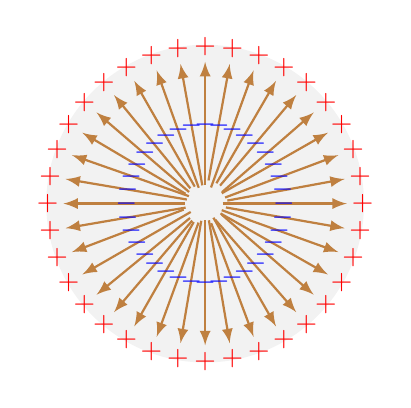
\begin{tikzpicture}[>=latex]
					\pgfmathsetseed{1}
					\draw[fill=gray!5, line width=1pt, gray!10] (0, 0) circle (2);
					\foreach \a in {10,20,...,360} {
							\draw[thick, ->, brown] (\a:{0.2 + 0.1*rnd}) -- (\a:1.8);
							\node[text=red]  at (\a:2) {$+$};
							\node[text=blue] at (\a:1) {$-$};
						}
				\end{tikzpicture}
			\end{column}
			\begin{column}{0.6\linewidth}
				\begin{overprint}
					\onslide<2>
					\begin{block}{}\justifying
						Якщо в результаті поляризації на  зовнішню поверхню виходить заряд $q =
							\oiint\limits_S
							\sigma' dS$, то в об'ємі речовини залишається заряд протилежного знаку.
						Оскільки
						речовина не заряджена, то
						\begin{equation*}
							\oiint\limits_S \sigma' dS = - \iiint\limits_V \rho' dV.
						\end{equation*}
					\end{block}
					\onslide<3>
					\begin{block}{}
						Оскільки $ 	\oiint\limits_S \sigma' dS = \oiint\limits_S P_n dS$, то
						\begin{equation*}
							\tcbhighmath{
								\oiint\limits_S P_n dS = - \iiint\limits_V \rho' dV.
							}
						\end{equation*}
						Цей вираз складає \alert{теорему Гаусса для вектора поляризації}.
					\end{block}
					\onslide<4>
					\begin{block}{}
						Теорема Гаусса в диференціальній форму
						\begin{equation*}
							\tcbhighmath{
								\divg\vect{P} = - \rho'.
							}
						\end{equation*}
						У окремому випадку однорідної поляризації, коли $\vect{P} = \const$, маємо
						$\rho' = 0$.
					\end{block}
				\end{overprint}
			\end{column}
		\end{columns}

	\end{onlyenv}
\end{frame}
% ===========================================================================




% ============================== Слайд ## ===================================
\begin{frame}{Вектор електричної індукції $\vect{D}$}{}\small
	\begin{onlyenv}<1>
		\begin{block}{}\justifying
			Електричне поле в створюють не лише вільні, а і поляризаційні заряди. У загальному випадку в
			теоремі Гаусса для вектора $\Efield$ слід врахувати наявність не тільки вільних, а й
			зв'язаних (поляризаційних) зарядів:
			\begin{equation*}
				\divg\Efield = 4\pi(\rho + \rho').
			\end{equation*}
			Оскільки $\divg\vect{P} = - \rho'$ , отримуємо $\divg\Efield = 4\pi(\rho -\divg\vect{P})$:
			\begin{equation*}
				\tcbhighmath{
					\Dfield = \Efield + 4\pi\vect{P}.
				}
			\end{equation*}
		\end{block}
		\begin{block}{}
			Теорема Гаусса для електричного поля в речовині набуде вигляду:
			\begin{equation*}
				\divg\Dfield = 4\pi\rho.
			\end{equation*}
		\end{block}
	\end{onlyenv}
	\begin{onlyenv}<1-2>
		\begin{block}{}
			Введений у вектор $\Dfield$ називається \alert{вектором електричної індукції}.
		\end{block}
	\end{onlyenv}
	\begin{onlyenv}<2>
		\begin{block}{}
			\begin{equation*}
				\tcbhighmath{
					\Dfield = \Efield + 4\pi\vect{P}.
				}
			\end{equation*}
			Теорема Гаусса для електричного поля в речовині:
		\end{block}
		\begin{columns}
			\begin{column}{0.5\linewidth}
				\begin{block}{}\centering
					в диференціальній формі
					\begin{equation*}
						\tcbhighmath{\divg\Dfield = 4\pi\rho.}
					\end{equation*}
				\end{block}
			\end{column}
			\begin{column}{0.5\linewidth}
				\begin{block}{}\centering
					в інтегральній формі
					\begin{equation*}
						\tcbhighmath{\oiint\limits_S\Dfield = 4\pi\iiint\limits_V \rho dV.}
					\end{equation*}
				\end{block}
			\end{column}
		\end{columns}
		\begin{block}{}\justifying
			У формулювання теореми Гаусса для поля в речовині \alert{входять тільки вільні заряди}.
			Поляризаційні ж заряди враховані у визначенні вектора індукції $\Dfield$.
		\end{block}
	\end{onlyenv}
\end{frame}
% ===========================================================================


% ============================== Слайд ## ===================================
\begin{frame}{Діелектрична проникність}{}
	\begin{block}{}
		Для діелектриків для яких справедливо співвідношення $\vect{P} = \chi\Efield$:
		\begin{equation*}
			\Dfield = \Efield + 4\pi\vect{P} = (1 + 4\pi\chi) \Efield =   \epsilon\Efield, \quad
			\tcbhighmath{\Dfield = \epsilon\Efield.}
		\end{equation*}
		де
		$
			\tcbhighmath{
				\epsilon = 1 + 4\pi\chi.
			}
		$
		називається \alert{діелектричною проникністю середовища}. Для випадку постійних електричних полів
		виявляється $\chi > 0$, а тому і $\epsilon > 0$.
	\end{block}
	\begin{columns}
		\begin{column}{0.25\linewidth}\centering
			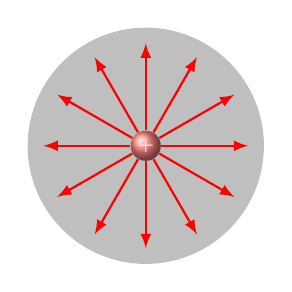
\begin{tikzpicture}[>=latex]
				\fill[gray!50] (0, 0) circle (1.5);
				\node[circle, ball color=red!50, inner sep=1pt, text=white, font=\scriptsize] (Q) at (0,0)
				{$+$};
				\foreach \a in {0,30,...,330} {
						\draw[thick, ->, red] (Q) -- (\a:1.3);
					}
			\end{tikzpicture}
		\end{column}
		\begin{column}{0.75\linewidth}
			\begin{block}{}\justifying\footnotesize
				Розглянемо точковий заряд $Q$ вміщений в нескінченний діелектрик з проникністю
				$\epsilon$.
				Скориставшись теоремою Гаусса для вектора $\Dfield$ знайдемо поле в діелектрику:
				\begin{equation*}
					\Efield = \frac{Q}{\epsilon r^3}\vect{r}.
				\end{equation*}
				Оскільки $\epsilon > 1$, то поле слабкіше ніж у вакуумі. Тобто,
				\alert{поляризаційні заряди призводять до ослаблення поля}.
			\end{block}
		\end{column}
	\end{columns}
\end{frame}
% ===========================================================================




% ============================== Слайд ## ===================================
\begin{frame}{Граничні умови в присутності діелектриків}{}
	\begin{onlyenv}<1>
		\begin{columns}
			\begin{column}{0.6\linewidth}
				\begin{block}{}\scriptsize\justifying
					Застосуємо теорему Гауса до нескінченно малого циліндра, що охоплює частину межі
					розділу двох
					середовищ. Вважаючи $d\vect{S}_1 = - d\vect{S}_2$, $q = \sigma dS$,
					$d\vect{S}_1 =
						\vect{n}\ dS$,
					маємо
				\end{block}
			\end{column}
			\begin{column}{0.4\linewidth}\centering
				 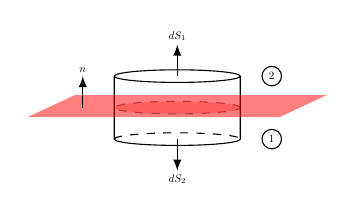
\begin{tikzpicture}[
scale=0.4,
transform shape,
>=latex,
declare function = {
h = 2;
r=2;
r2=0.2;
},
]

\fill[red!50, opacity=0.5, draw=black, dashed] (0,1) circle (r and r2);
\draw (-2,h) -- (-2,0) arc (180:360:r and r2) -- (2,h) ++ (-2,0) circle (r and r2);
\draw[dashed] (-2,0) arc (180:0:r and r2);
\fill[red,opacity=0.5]
 (-4.75,0.7) -- ++(8,0) -- ++(1.5,0.7) -- ++(-8,0) ;
\draw[->] (0,h) -- ++(0,1) node[above] {$d\vect{S}_1$};
\draw[->] (0,0) -- ++(0,-1) node[below] {$d\vect{S}_2$};

\draw[->] (-3,1) -- ++(0,1) node[above] {$\vect{n}$};

\node[circle, draw] at (3,0) {$1$};
\node[circle, draw] at (3,h) {$2$};
\end{tikzpicture}
			\end{column}
		\end{columns}
		\begin{block}{}\scriptsize
			\begin{equation*}
				\oiint_S \Dfield\cdot d\vect{S} = 4\pi\sigma\ \Rightarrow  \Dfield\cdot
				d\vect{S}_1 +
				\Dfield\cdot d\vect{S}_2 = 4\pi\sigma dS
			\end{equation*}
		\end{block}
		\begin{block}{}
			Звідси випливає перша гранична умова:
			\begin{equation*}
				\tcbhighmath{
					D_{1n} - D_{2n} = 4\pi\sigma.
				}
			\end{equation*}
		\end{block}
		\begin{alertblock}{}\justifying\scriptsize
			Нормальна складова вектора $\Dfield$ зазнає стрибка при
			переході через границю розділу діелектриків, якщо на ній є вільні заряди. Якщо вільних
			зарядів на границі розділу нема, то $D_{1n} = D_{2n}$ і стрибка не буде.
		\end{alertblock}
	\end{onlyenv}
	\begin{onlyenv}<2>
		\begin{columns}
			\begin{column}{0.6\linewidth}
				\begin{block}{}\scriptsize\justifying
					Застосуємо теорему про циркуляцію до нескінченно малого прямокутного
					контуру $L$, що проходить на нескінченно малій відстані над і під поверхнею
					розділу середовищ. Вважаючи, що $d\vect{r}_1 = -d\vect{r}_2$, маємо
				\end{block}
			\end{column}
			\begin{column}{0.4\linewidth}\centering
				 \begin{tikzpicture}[
scale=0.4,
transform shape,
>=latex,
declare function = {
h = 2;
r=2;
r2=0.2;
},
midarrow/.style={%
   postaction={ decorate,transform shape,
   decoration={ markings, mark=at position .5 with {\arrow{>}}}}},
]

\fill[red,opacity=0.5]
 (-4.75,0.7) -- ++(8,0) -- ++(1.5,0.7) -- ++(-8,0) ;

\draw[midarrow] (2, 1) -- ++(0, 1) -- node[above=5pt] {$L$} ++(-4, 0) -- ++(0, -1);
\draw[midarrow] (-2, 1) -- ++(0, -1) -- ++(4, 0) -- ++(0, 1);

\draw[->] (-3,1) -- ++(-2,0) node[above] {$\vect{\tau}$};
\draw[->] (-3,1) -- ++(0,1) node[above] {$\vect{n}$};
\draw[->] (-3,1) -- ++({180+45}:1) node[below] {$\vect{b}$};
\node[circle, draw] at (3,0) {$1$};
\node[circle, draw] at (3,h) {$2$};
\end{tikzpicture}
			\end{column}
		\end{columns}
		\begin{block}{}\scriptsize
			\begin{equation*}
				\oint\limits_L \Efield\cdot d\vect{r} = 0 \Rightarrow \Efield_1 d\vect{r}_1 +
				\Efield_2 d\vect{r}_2 = 0
			\end{equation*}
		\end{block}
		\begin{block}{}
			Звідси випливає друга гранична умова:
			\begin{equation*}
				\tcbhighmath{
					E_{1\tau} = E_{2\tau}.
				}
			\end{equation*}
		\end{block}
		\begin{alertblock}{}\justifying\scriptsize
			Тангенціальна складова $\Efield$ виявляється однаковою по обидва боки границі розділу
			(не
			зазнає стрибка).
		\end{alertblock}
	\end{onlyenv}
\end{frame}
% ===========================================================================


% ============================== Слайд ## ===================================
\begin{frame}{Заломлення силових ліній на границі діелектрика}{}\small
	\begin{block}{}\justifying
		Лінії векторів $\Efield$ і $\Dfield$ на границі розділу двох
		діелектриків заломлюються.
	\end{block}
	\begin{columns}
		\begin{column}{0.55\linewidth}\centering
			\begin{tikzpicture}[>=latex,
					scale=0.75,
					transform shape,
					pencildraw/.style={ %
							decorate,
							decoration={random steps,segment length=3pt,amplitude=2pt}
						},
				]



				% Георметрія

				% Середовище 1
				\fill[thick, red!10,  pencildraw, opacity=0.85] (-2, +0.05) rectangle (6, -2.1);
				\node[circle, draw, inner sep =1pt, font=\scriptsize] at (-1.8, -0.5) {$1$};

				% Середовище 2
				\fill[thick, blue!10, pencildraw, opacity=0.85] (-2, -0.05) rectangle (6, +2.1);
				\node[circle, draw, inner sep =1pt, font=\scriptsize] at (-1.8, +0.5) {$2$};

				% Границя розділу
				\draw[line width=2pt, gray!50] (-2, 0) -- (6, 0);

				\draw[dashed] (-1, -2) -- ++(0, 4);

				\draw[midarrow] (-1.5, -2) -- (-1,0);
%				\draw[->, red, thin, opacity=0.5] (-1.5, 0) -- node[above, font=\scriptsize]
%				{$E_{1\tau}$}
%				++(0.5, 0);
%				\draw[->, red, thin, opacity=0.5] (-1.5, -2) -- node[left, font=\scriptsize]
%				{$E_{1n}$} ++(0, 2);
%
%				\draw[->, red, thin, opacity=0.5] (-1, 0)     -- node[above, font=\scriptsize]
%				{$E_{2\tau}$}
%				++(1, 0);
%				\draw[->, red, thin, opacity=0.5] (0, 0)      -- node[right, font=\scriptsize]
%				{$E_{2n}$} ++(0,
%				2);

				\draw[midarrow] (-1,0) -- ++(1, 2);
				\draw (-1,0) ++(90:0.8) arc[start angle=90, delta angle={-atan(1/2)}, radius =
						0.8]  node[pos=0.5, anchor=south, inner sep=1, font=\scriptsize] {$\alpha_2$};
				\draw (-1,0) ++(-90:0.8) arc[start angle=-90, delta angle={-atan(0.5/2)}, radius =
						0.8] node[pos=0.5, anchor=north, inner sep=5pt, font=\scriptsize] {$\alpha_1$};

				% Поле вектора E
				\foreach[] \x in {0,1,...,6}{
						\draw[midarrow, red] (0.25*\x, -2) -- ++(0.5, 2);
						\ifnum\x<4
							\draw[midarrow, red] ({0.5*(\x + 1)}, 0) -- ++(1, 2);
						\fi
					}
				\node[font=\small] at (0.8, -2.5) {Поле вектора $\Efield$};

				% Поле вектора D
				\begin{scope}[xshift=3cm]
					\foreach[] \x in {0,1,...,6}{
							\draw[midarrow, blue ] (0.25*\x, -2) -- ++(0.5, 2);
							\draw[midarrow, blue ] ({0.25*(\x+2)}, 0) -- ++(1, 2);
						}
				\end{scope}
				\node[font=\small] at (3.8, -2.5) {Поле вектора $\Dfield$};

			\end{tikzpicture}
		\end{column}
		\begin{column}{0.45\linewidth}\scriptsize
			Граничні умови для вектора $\Efield$
			\begin{equation*}
				\begin{cases}
					E_{1\tau} = E_{2\tau},\ \Rightarrow\ E_1\sin\alpha_1 = E_2\sin\alpha_2, \\
					D_{1n} = D_{2n},\ \Rightarrow\ \epsilon_1E_1\cos\alpha_1 =
					\epsilon_2E_2\cos\alpha_2
				\end{cases}
			\end{equation*}
			Граничні умови для вектора $\Dfield$
			\begin{equation*}
				\begin{cases}
					E_{1\tau} = E_{2\tau},\ \Rightarrow\ D_1/\epsilon_1\sin\alpha_1 =
					D_2/\epsilon_2\sin\alpha_2, \\
					D_{1n} = D_{2n},\ \Rightarrow\ D_1\cos\alpha_1 =
					D_2\cos\alpha_2
				\end{cases}
			\end{equation*}
		\end{column}
	\end{columns}
	\begin{block}{}\justifying
		Закон заломлення ліній $\Efield$ та $\Dfield$ однаковий:
		\begin{equation*}
			\tg\alpha_2 / \tg\alpha_1 = \epsilon_2 / \epsilon_1.
		\end{equation*}
		В діелектрику з більшим значенням $\epsilon$ лінії $\Efield$ і $\Dfield$
		становитимуть більший кут із нормаллю до границі розділу.
	\end{block}
\end{frame}
% ===========================================================================


%% ============================== Слайд ## ===================================
%\begin{frame}{Заряди на поверхні провідник-діелектрик}{}
%
%\end{frame}
%% ===========================================================================

%% --------------------------------------------------------
\section{Теорія діелектричної проникності}
%% --------------------------------------------------------


% ============================== Слайд ## ===================================
\begin{frame}{Теорія діелектричної проникності полярних діелектриків}{}
	\begin{onlyenv}<1-2>
		\begin{center}
			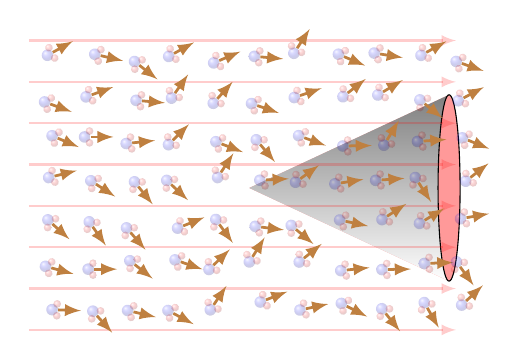
\begin{tikzpicture}[>=latex, scale=0.7, transform shape]
				\pgfmathsetseed{1}
				\tikzset{
					water/.pic={
							\begin{scope}[opacity=0.2]
								\node[circle, ball color=blue, inner sep=0, minimum size=0.3cm] (O) at
								(0,0) {};
								\node[circle, ball color=red, inner sep=0, minimum size=0.2cm] (H1) at
								(-50:0.2) {};
								\node[circle, ball color=red, inner sep=0, minimum size=0.2cm] (H2) at
								(50:0.2) {};
							\end{scope}
							\draw[-latex, brown, line width=1pt] (O) -- ++(0.75, 0);
						}
				}
				\begin{scope}
					\pgfmathsetmacro{\a}{25}
					\pgfmathsetmacro{\r}{4}
					\shade[fill=red!40] (0,0) -- ++(\a:\r) -- ++(0,{-2*\r*sin(\a)}) -- cycle;
					\draw[fill=red!40] (0:{\r*cos(\a)}) circle(0.2 and {-\r*sin(\a)});
				\end{scope}
				\foreach \y in {-3,...,4} {
						\draw[->, red, thick, opacity=0.2] (-4,{0.75*\y-0.325}) -- ++(7.75,0);
					}
				\foreach \x in {-5,...,5}
					{
						\foreach \y in {-3,...,3}{
								\pic[scale=0.7, transform shape, rotate={random(-60,60)}] at
								({0.75*\x+0.2*rnd},
								{0.75*\y+0.2*rnd}) {water};
							}
					}

			\end{tikzpicture}
		\end{center}
	\end{onlyenv}
	\vspace*{-2em}
	\begin{overprint}
		\onslide<1>
		\begin{block}{}\justifying\small
			За розподілом Больцмана, число молекул в одиничному тілесному куті, які напрямлені під кутом
			$\theta$ до поля $\Efield$:
			\begin{equation*}
				\frac{dN}{d\Omega} = n(\theta) = n_0e^{-\frac{U}{kT}} =
				n_0e^{+\frac{p_0E\cos\theta}{kT}}
				\approx  n_0\left(1 + \frac{p_0E\cos\theta}{kT}\right).
			\end{equation*}
			%		Вздовж поля ($\cos\theta = 1$) буде орієнтовано більше молекул, ніж проти
			%		поля ($\cos\theta = -1$).
		\end{block}
		\onslide<2-3>
		\begin{block}{}
			Поляризація (напрямлена вздовж поля):
			\begin{equation*}
				P =  n p_0 \overline{\cos\theta} = n p_0 \left( \frac 1N \int \cos\theta d N\right)  =
				\frac{n
					p_0^2}{3kT}E
			\end{equation*}
		\end{block}
	\end{overprint}
	\begin{onlyenv}<3>
		\begin{block}{}\justifying
			Оскільки поляризація $P = \chi E$ пропорційна полю $E$, тому  поляризовність:
			\begin{equation*}
				\chi = \frac{n p_0^2}{3kT}. \quad \epsilon = 1 + \frac{4\pi np_0^2}{3kT}.
			\end{equation*}
			обернено пропорційна температурі $\chi \sim \frac1T$. Ця залежність виду називається \alert{законом
				Кюрі}. Якщо діелектрична проникність діелектрика залежить від температури, це означає, що
			діелектрик складається із полярних молекул.
		\end{block}
	\end{onlyenv}
\end{frame}
% ===========================================================================



%% --------------------------------------------------------
\section{Типи діелектриків}
%% --------------------------------------------------------



% ============================== Слайд ## ===================================
\begin{frame}{Типи діелектриків}{Електрети}
	\begin{onlyenv}<1>
		\begin{block}{}\justifying
			Електрети --- це діелектрики, які тривалий час зберігають поляризацію після зняття
			зовнішнього поля. Електрет є <<\alert{електричним аналогом постійного магніту}>>.
		\end{block}
		\tikzset{
			cylinder/.pic={
					\begin{scope}
						\node[cylinder,draw=black,thick,aspect=0.5,minimum height=2cm,minimum
							width=1.5cm,shape
							border rotate=90,cylinder uses custom fill, cylinder body
							fill=red!30,cylinder end
							fill=red!10] (A) {}; \draw[dashed] let \p1 = ($ (A.after bottom) -
							(A.before bottom) $),
						\n1 = {0.5*veclen(\x1,\y1)-\pgflinewidth}, \p2 = ($ (A.bottom) - (A.after
							bottom)!.5!(A.before bottom) $), \n2 = {veclen(\x2,\y2)-\pgflinewidth}
						in
						([xshift=-\pgflinewidth] A.before bottom) arc [start angle=0, end
								angle=180, x
								radius=\n1, y radius=\n2];
					\end{scope}
				}
		}
		%=========================================================
		\begin{figure}[h!]\centering
			%---------------------------------------------------------
			\begin{subfigure}[t]{0.45\linewidth}\centering
				\begin{tikzpicture}[>=latex, scale=0.75, transform shape]
					\pic at (0,0) {cylinder};
					\node[text=red, circle, inner sep=1pt,  font=\scriptsize, above] at (0, 1)
					{$+$};
					\node[text=blue, circle, inner sep=1pt, font=\scriptsize, below] at (0, -1)
					{$-$};
					\foreach[count=\c from 0] \x in {0.85, 0.75, 0.70} {
							\draw[midarrow, blue] (-\x,0) ellipse({0.8-0.2*\c} and {2.5-0.5*\c});
							\draw[midarrowR, blue, rotate around={180:(\x,0)}] (\x,0)
							ellipse({0.8-0.2*\c}
							and
								{2.5-0.5*\c});
						}
				\end{tikzpicture}
				\caption{\centering Поле вектора електричної індукції $\Dfield$}
			\end{subfigure}
			%---------------------------------------------------------
			\begin{subfigure}[t]{0.45\linewidth}\centering
				\begin{tikzpicture}[>=latex, scale=0.75, transform shape]
					\foreach[count=\c from 0] \x in {0.85, 0.75, 0.70} {
							\draw[midarrow, red] (-\x,0) ellipse({0.8-0.2*\c} and {2.5-0.5*\c});
							\draw[midarrowR, red, rotate around={180:(\x,0)}] (\x,0)
							ellipse({0.8-0.2*\c}
							and
								{2.5-0.5*\c});
						}
					\pic[] at (0,0) {cylinder};
					\node[text=red, circle, inner sep=1pt,  font=\scriptsize, above] at (0, 1)
					{$+$};
					\node[text=blue, circle, inner sep=1pt, font=\scriptsize, below] at (0, -1)
					{$-$};
					\begin{scope}
						\clip (-0.75, -0.875) -- ++(0, 1.86) -- ++(1.5, 0) -- ++(0, -1.86) -- cycle;
						\foreach[count=\c from 1] \x in {0.85, 0.75, 0.70} {
								\foreach \m in {-1,1} {
										\draw[midarrow, red, xscale=\m] (0,0) ellipse({0.8-0.2*\c}
										and
											{2.6-0.5*\c});
									}
							}
					\end{scope}
				\end{tikzpicture}
				\caption{\centering Поле вектора напруженості електричного поля $\Efield$}
			\end{subfigure}
			%---------------------------------------------------------
		\end{figure}
		%=========================================================
	\end{onlyenv}
	\begin{onlyenv}<2>
		\tikz[remember picture,overlay] \node[opacity=0.5,inner sep=0pt,
			anchor=north east] at (current page.north
		east){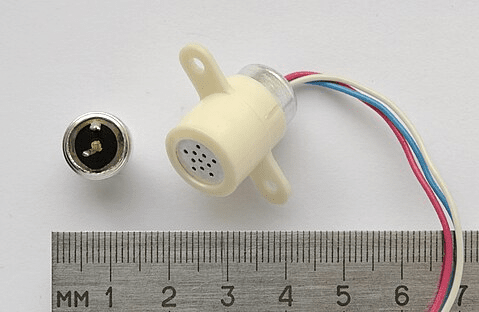
\includegraphics[width=3cm]{Electret_microphone}};
		\begin{block}{}\justifying
			Електрети можна виготовити, нагріваючи діелектрик і піддаючи його впливу
			сильного поля $\Efield$, так що полярні молекули вистоюються за полем.

			\bigskip

			Якщо потім діелектрик
			охолодити, то поляризація речовини тривалий час зберігається, оскільки поворот молекул у
			затверділій речовині ускладнений. У результаті отримують \alert{<<заморожену>>
				поляризацію}.
		\end{block}

		\begin{block}{}\justifying\scriptsize
			Кварц та інші форми діоксиду кремнію є природними електретами. Сьогодні більшість
			електретів виготовляють із синтетичних полімерів, наприклад, фторопластів,
			поліпропілену,
			поліетилентерефталату (ПЕТ) тощо.
		\end{block}
	\end{onlyenv}
\end{frame}
% ===========================================================================



% ============================== Слайд ## ===================================
\begin{frame}{Типи діелектриків}{Сегнетоелектрики}
	\begin{block}{}\justifying
		\alert{Сегнетоелектрик} --- це кристалічний діелектрик, який має \alert{спонтанну поляризацію
			всередині окремих доменів}, яка виникає без зовнішнього електричного поля. Під впливом поля
		домени переорієнтуються, змінюючи загальну поляризацію матеріалу.
	\end{block}

	\begin{columns}
		\begin{column}{0.7\linewidth}
			\begin{block}{}\justifying\small
				\alert{Домен} --- це локальна область усередині сегнетоелектрика, де дипольні моменти
				орієнтовані в одному й тому самому напрямку. У кожному домені поляризація постійна і спрямована
				в один бік. Розміри від кількох до сотень мікрометрів.
			\end{block}
		\end{column}
		\begin{column}{0.3\linewidth}\centering
			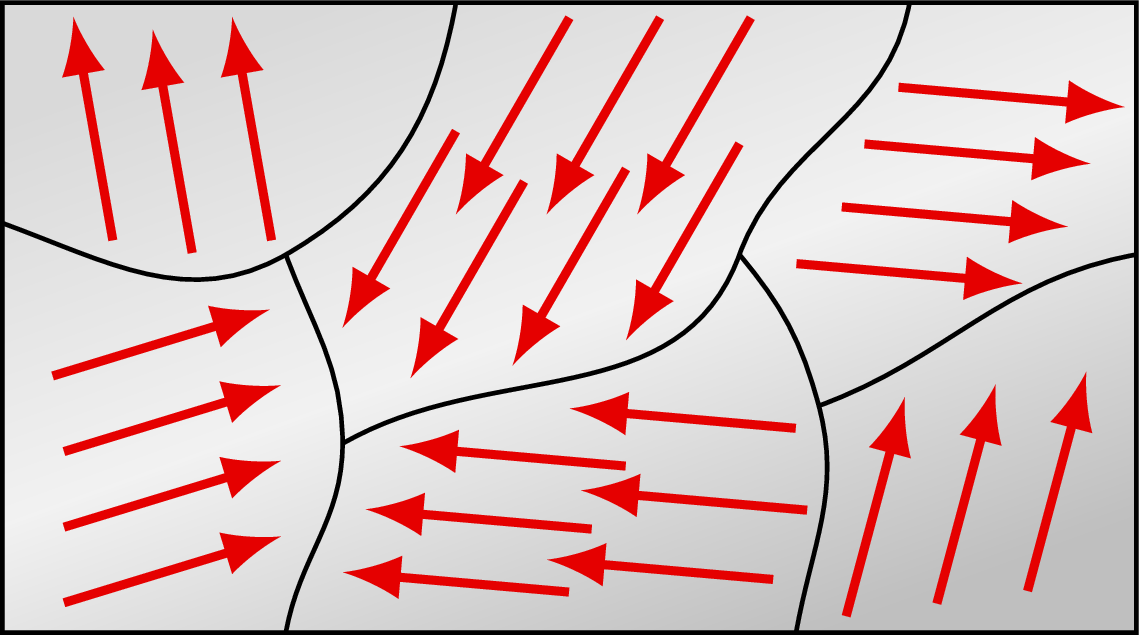
\includegraphics[width=1\linewidth]{domains}
		\end{column}
	\end{columns}


	\begin{block}{}\scriptsize\justifying
		Відомі сегнетоелектрики.
		\begin{itemize}
			\item Титанат барію (\ce{BaTiO3}).
			\item Сегнетова сіль (\ce{KNaC4H4O6*4H2O})
		\end{itemize}
		Застосування сегнетоелектриків пов'язані з аномально великими значеннями $\epsilon$
		(конденсатори, вариконди). Використовуються у створенні електромеханічних і механоелектричних
		перетворювачів у широкому діапазоні частот, датчики мікропереміщень, гідрофони, акселерометри,
		стабілізатори частоти тощо.
	\end{block}


	%\begin{block}{}
	%    Порівняно з ізотропними діелектриками, сегнетоелектрики мають відмінні властивості:
	%    \begin{enumerate}\small
	%        \item анізотропія властивостей --- залежність діелектричної проникності від напрямку;
	%        \item надвисокі значення діелектричної проникності до $\sim 10^4$;
	%        \item залежність діелектричної проникності ε від температури і напруженості електричного
	%        поля;
	%        \item нелінійна залежність вектора поляризації від напруженості електричного поля;
	%        \item наявність діелектричного гістерезису.
	%    \end{enumerate}
	%\begin{block}{}
	%    Такі властивості сегнетоелектриків спостерігаються лише в певному інтервалі температур менших
	%    за температури Кюрі $T < T_K$. Для кожного сегнетоелектрика існує своє значення температури
	%    Кюрі.
	%\end{block}
	%\end{block}
	% https://studfile.net/preview/17697221/
\end{frame}
% ===========================================================================



% ============================== Слайд ## ===================================
\begin{frame}{Гістерезис в сегнетоелектриках}{}\small
	\begin{block}{}\justifying
		\alert{Гістерезис} --- неоднозначна петлеподібна залежність поляризації сегнетоелектриків від
		зовнішнього електричного поля $\Efield$ за його циклічної зміни.
	\end{block}
	\begin{columns}
		\begin{column}{0.5\linewidth}\centering
			\begin{tikzpicture}[>=latex, scale=0.8, transform shape,
					point/.style={circle, draw, inner sep=0.7pt, fill=white}
				]

				\draw[-latex, name path=E] (-2.5,0) -- (2.5,0) node[below]{$E$};
				\draw[-latex, name path
					=P] (0,-1.5) -- (0,1.5)node[left]{$P$};

				\draw[samples=200, domain=-3:2, name path=d, midarrow,  red, thick] plot ({\x+0.5}, {0.2*\x
						+ tanh(1.9*\x) + 0.1}); \draw[samples=200, domain=-2:3, name path=u, midarrowR, red, thick]
				plot ({\x-0.5}, {0.2*\x + tanh(1.9*\x) - 0.1});
				\draw[midarrow, thick, cyan!50!black] (0,0) .. controls (0.5, 0.2) and
				(0.2, 1.0) ..
				(1.52, 1.28);
				\tikzfillbetween[of=u and d]{blue, opacity=0.1};

				\foreach \i/\a in {P/u, P/d, E/u, E/d} {
						\path[name intersections={of={\i} and {\a}}]
						(intersection-1) node[point] (\i\a) {};
					}
				\node[left,  text=brown] at (Pu) {$P_r$};
				\node[right, text=brown] at (Pd) {$-P_r$};
				\node[above left, text=red] at (Eu) {$-E_c$};
				\node[below right, text=red] at (Ed) {$E_c$};
			\end{tikzpicture}
		\end{column}
		\begin{column}{0.8\linewidth}
			\begin{figure}
				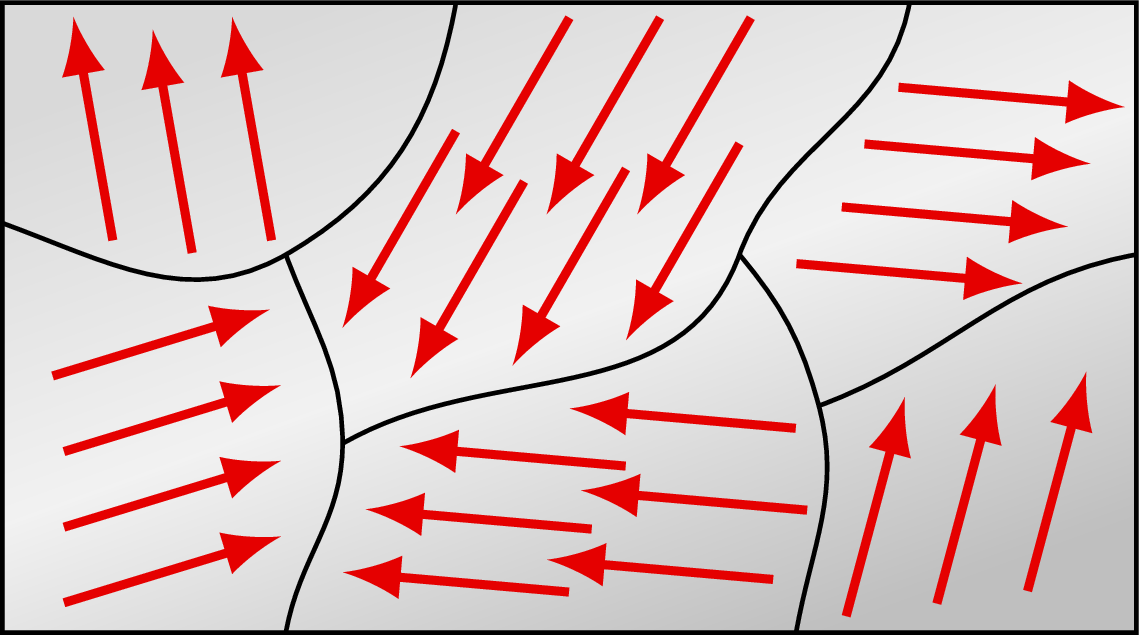
\includegraphics[width=0.5\linewidth]{domains}
				\caption{\centering\scriptsize Доменна структура сегнетоелектрика}
			\end{figure}
		\end{column}
	\end{columns}
	\begin{enumerate}\justifying\scriptsize
		\item За високого електричного поля $ E $, поляризація досягає насичення і поводить себе як
		      діелектрик у якого $P \propto E$.
		\item  Поле зменшується до нуля $E = 0$, але поляризація $ P_r $ залишається.
		\item Для того щоб звести поляризацію до нуля, потрібно прикласти негативне поле $-E_c$,
		      яке називається \alert{коерцитивною силою}.
		\item При подальшому збільшенні негативного поля поляризація $P \propto E$.
		\item  При зменшенні негативного поля до нуля поляризація залишається на рівні $ -P_r $.
	\end{enumerate}
\end{frame}
% ===========================================================================



% ============================== Слайд ## ===================================
\begin{frame}{Типи діелектриків}{П'єзоелектрики та піроелектрики}
	\begin{block}{}\justifying
		\alert{П'єзоелектрики} --- діелектрики, що можуть або під дією деформації індукувати
		електричний заряд на своїй поверхні (прямий п'єзоефект), або під впливом зовнішнього
		електричного поля деформуватися (зворотний п'єзоефект).
	\end{block}

	\begin{block}{}\justifying
		\alert{Піроелектрики} --- кристалічні діелектрики, що мають спонтанну поляризацію, тобто
		поляризацією за відсутності зовнішніх впливів. міна спонтанної поляризації та поява
		електричного поля в піроелектриках відбувається при зміні температури, а також при
		деформуванні. Таким чином, усі піроелектрики є п'єзоелектриками, але не всі п'єзоелектрики
		мають піроелектричний ефект.
	\end{block}
\end{frame}
% ===========================================================================



% ============================== Слайд ## ===================================
\begin{frame}{Підсумки}{}\small
\begin{tblr}{
colspec={Q[c,l]Q[mode=dmath]}
}
Вектор поляризації & \vect{P} = \frac1V\sum \vect{p}_i \\
Для лінійних діелектриків & \vect{P} = \chi \Efield \\
Теорема Гаусса для вектора $\vect{P}$ & \oiint\limits_S \vect{P}d\vect{S} = - \iiint\limits_V\rho'
dV\\
в диференціальній формі & \divg\vect{P} = - \rho' \\
Вектор електричної індукції & \Dfield = \Efield  + 4\pi\vect{P}\\
Для лінійних діелектриків & \Dfield = \epsilon\Efield \\
{Зв'язок проникності і поляризовності \\ (для лінійних діелектриків)} & \epsilon = 1+ 4\pi\chi \\
{ Поляризовність полярних діелектриків \\ (закон Кюрі) } & \chi \propto T^{-1} \\
Теорема Гаусса в діелектриках & \oiint\limits_S \vect{D}d\vect{S} = 4\pi \iiint\limits_V\rho dV \\
в диференціальній формі & \divg\Dfield = 4\pi\rho
\end{tblr}
\end{frame}
% ===========================================================================

\end{document}
